\documentclass[a4]{article}
\pagestyle{myheadings}

%%%%%%%%%%%%%%%%%%%
% Packages/Macros %
%%%%%%%%%%%%%%%%%%%
\usepackage{mathrsfs}


\usepackage{fancyhdr}
\pagestyle{fancy}
\lhead{}
\chead{}
\rhead{}
\lfoot{}
\cfoot{} 
\rfoot{\normalsize\thepage}
\renewcommand{\headrulewidth}{0pt}
\renewcommand{\footrulewidth}{0pt}
\newcommand{\RomanNumeralCaps}[1]
    {\MakeUppercase{\romannumeral #1}}

\usepackage{amssymb,latexsym}  % Standard packages
\usepackage[utf8]{inputenc}
\usepackage[russian]{babel}
\usepackage{MnSymbol}
\usepackage{mathrsfs}
\usepackage{amsmath,amsthm}
\usepackage{indentfirst}
\usepackage{graphicx}%,vmargin}
\usepackage{graphicx}
\graphicspath{{pictures/}} 
\usepackage{verbatim}
\usepackage{color}
\usepackage[nottoc,numbib]{tocbibind}
\usepackage{float}

\usepackage{listings}
\definecolor{codegreen}{rgb}{0,0.6,0}
\definecolor{codegray}{rgb}{0.5,0.5,0.5}
\definecolor{codepurple}{rgb}{0.58,0,0.82}
\definecolor{backcolour}{rgb}{0.95,0.95,0.92}
 
\lstdefinestyle{mystyle}{
    backgroundcolor=\color{backcolour},   
    commentstyle=\color{codegreen},
    keywordstyle=\color{magenta},
    numberstyle=\tiny\color{codegray},
    stringstyle=\color{codepurple},
    basicstyle=\footnotesize,
    breakatwhitespace=false,         
    breaklines=true,                 
    captionpos=b,                    
    keepspaces=true,                 
    numbers=left,                    
    numbersep=5pt,                  
    showspaces=false,                
    showstringspaces=false,
    showtabs=false,                  
    tabsize=2
}
 
\lstset{style=mystyle}

\usepackage{url}
\urldef\myurl\url{foo%.com}





\DeclareGraphicsExtensions{.pdf,.png,.jpg}% -- настройка картинок

\usepackage{epigraph} %%% to make inspirational quotes.
\usepackage[all]{xy} %for XyPic'a
\usepackage{color} 
\usepackage{amscd} %для коммутативных диграмм
%\usepackage[colorlinks,urlcolor=red]{hyperref}

%\renewcommand{\baselinestretch}{1.5}
%\sloppy
%\usepackage{listings}
%\lstset{numbers=left}
%\setmarginsrb{2cm}{1.5cm}{1cm}{1.5cm}{0pt}{0mm}{0pt}{13mm}


\newtheorem{Lemma}{Лемма}[section]
\newtheorem{Proposition}{Предложение}[section]
\newtheorem{Theorem}{Теорема}[section]
\newtheorem{Corollary}{Следствие}[section]
\newtheorem{Remark}{Замечание}[section]
\newtheorem{Definition}{Определение}[section]
\newtheorem{Designations}{Обозначение}[section]




%%%%%%%%%%%%%%%%%%%%%%% 
%Подготовка оглавления% 
%%%%%%%%%%%%%%%%%%%%%%% 
\usepackage[titles]{tocloft}
\renewcommand{\cftdotsep}{2} %частота точек
\renewcommand\cftsecleader{\cftdotfill{\cftdotsep}}
\renewcommand{\cfttoctitlefont}{\hspace{0.38\textwidth} \LARGE\bfseries} 
\renewcommand{\cftsecaftersnum}{.}
\renewcommand{\cftsubsecaftersnum}{.}
\renewcommand{\cftbeforetoctitleskip}{-1em} 
\renewcommand{\cftaftertoctitle}{\mbox{}\hfill \\ \mbox{}\hfill{\footnotesize Стр.}\vspace{-0.5em}} 
%\renewcommand{\cftchapfont}{\normalsize\bfseries \MakeUppercase{\chaptername} } 
%\renewcommand{\cftsecfont}{\hspace{1pt}} 
\renewcommand{\cftsubsecfont}{\hspace{1pt}} 
%\renewcommand{\cftbeforechapskip}{1em} 
\renewcommand{\cftparskip}{3mm} %определяет величину отступа в оглавлении
\setcounter{tocdepth}{5} 
\renewcommand{\listoffigures}{\begingroup %добавляем номер в список иллюстраций
\tocsection
\tocfile{\listfigurename}{lof}
\endgroup}
\renewcommand{\listoftables}{\begingroup %добавляем номер в список иллюстраций
\tocsection
\tocfile{\listtablename}{lot}
\endgroup}


   
   
%\renewcommand{\thelikesection}{(\roman{likesection})}
%%%%%%%%%%%
% Margins %
%%%%%%%%%%%
\addtolength{\textwidth}{0.7in}
\textheight=630pt
\addtolength{\evensidemargin}{-0.4in}
\addtolength{\oddsidemargin}{-0.4in}
\addtolength{\topmargin}{-0.4in}

%%%%%%%%%%%%%%%%%%%%%%%%%%%%%%%%%%%
%%%%%%Переопределение chapter%%%%%% 
%%%%%%%%%%%%%%%%%%%%%%%%%%%%%%%%%%%
\newcommand{\empline}{\mbox{}\newline} 
\newcommand{\likechapterheading}[1]{ 
\begin{center} 
\textbf{\MakeUppercase{#1}} 
\end{center} 
\empline} 

%%%%%%%Запиливание переопределённого chapter в оглавление%%%%%% 
\makeatletter 
\renewcommand{\@dotsep}{2} 
\newcommand{\l@likechapter}[2]{{\bfseries\@dottedtocline{0}{0pt}{0pt}{#1}{#2}}} 
\makeatother 
\newcommand{\likechapter}[1]{ 
\likechapterheading{#1} 
\addcontentsline{toc}{likechapter}{\MakeUppercase{#1}}} 




\usepackage{xcolor}
\usepackage{hyperref}
\definecolor{linkcolor}{HTML}{000000} % цвет ссылок
\definecolor{urlcolor}{HTML}{AA1622} % цвет гиперссылок
 
\hypersetup{pdfstartview=FitH,  linkcolor=linkcolor,urlcolor=urlcolor, colorlinks=true}

%%%%%%%%%%%%
% Document %
%%%%%%%%%%%%

%%%%%%%%%%%%%%%%%%%%%%%%%%%%%
%%%%%%главы -- section*%%%%%%
%%%%section -- subsection%%%%
%subsection -- subsubsection%
%%%%%%%%%%%%%%%%%%%%%%%%%%%%%
\def \newstr {\medskip \par \noindent} 



\begin{document}
\def\contentsname{\LARGE{Содержание}}
\thispagestyle{empty}
\begin{center} 
\vspace{2cm} 
{\Large \sc Санкт-Петербургский Политехнический}\\
\vspace{2mm}
{\Large \sc Университет} им. {\Large\sc Петра Великого}\\
\vspace{1cm}
{\large \sc Институт прикладной математики и механики\\ 
\vspace{0.5mm}
\textsc{}}\\ 
\vspace{0.5mm}
{\large\sc Кафедра прикладной математики}\\
\vspace{15mm}
%\rule[0.5ex]{\linewidth}{2pt}\vspace*{-\baselineskip}\vspace*{3.2pt} 
%\rule[0.5ex]{\linewidth}{1pt}\\[\baselineskip] 
{\huge \sc Лабораторная работа №$4$\\
\vspace{4mm}
Эмпирические функции и ядерные оценки
\vspace{6mm}
 }
\vspace*{2mm}
%\rule[0.7ex]{\linewidth}{1pt}\vspace*{-\baselineskip}\vspace{3.2pt} 
%\rule[0.5ex]{\linewidth}{2pt}\\ 
\vspace{1cm}

{\sc $3$ курс$,$ группа $33631/2$}

\vspace{2cm} 
Студент \hfill Д. А. Плаксин\\
\vspace{1cm}
Преподаватель \hfill Баженов А. Н.\\
\vspace{20mm} 

\end{center} 
%\author{Я}
\begin{center}
\vfill {\large\textsc{Санкт-Петербург}}\\ 
2019 г.
\end{center}

%%%%%%%%%%%%%%%%%%%%%%%%%%%%%%%%%%%%%%%%%%%%%%%%%%%%%%%%%%%%%%%%%%%%%%%%%%%%%%%%%%%%%%%%%%%%%%
%\ \\[4cm]

%\rm
%%%%%%%%%%%%%%%%%%%%%%%%%%%%%%%%%%%%%%%%%%%%%%%%%%%%%%%%%%%%%%%%%%%%%%%%%%%%%%%%%%%%%%%%%%%%%%
\newpage
\pagestyle{plain}

%\begin{center}
%\begin{abstract} 

%\end{abstract}

%\end{center}

\newpage
\tableofcontents{}
\newpage
\listoffigures{}
\newpage

\section{Постановка задачи}

Для, приведённых ниже, пяти распределений сгенерировать выборки объёмом $20,\; 60,\; 100,$ для каждой выборки построить эмпирические функции распределения и ядерные оценки плотности распределения на отрезке $[-4, 4].$

Распределения \cite{distr_formulas}:
\begin{enumerate}
\item Стандартное нормальное распределение
\item Стандартное распределение Коши
\item Распределение Лапласа с коэффициентом масштаба $\sqrt{2}$ и нулевым коэффициентом сдвига.
\item Равномерное распределение на отрезке $\left[-\sqrt{3}, \sqrt{3}\right]$
\item Распределение Пуассона со значением матожидания равным двум.
\end{enumerate}

\section{Теория}
Эмпирическая функция распределения \cite{emp}, построенная по выборке $X = \left(X_1,\ldots, X_n\right)$ есть случайная функция $F_n(y),$ определённая на $\mathbb{R}:$
\begin{equation}
F_n(y) = \sum\limits_{i=1}^n I\left(X_i < y\right) \;\;\text{где}\; I\left(X_i < y\right) = \begin{cases} 
1, & X_i < y\\
0, & \text{иначе}
\end{cases}\hfill\label{eqn:emp}
\end{equation}

$X = \left(X_1,\ldots, X_n\right)$ есть одномерная выборка одинаково распределённых элементов, с плотностью распределения $f.$

Ядерная оценка плотности \cite{art}:
\begin{equation}
    f_h(x) = \frac{1}{nh}\sum\limits_{i=1}^nK\left(\frac{x-x_i}{h}\right)\label{eqn:art}
\end{equation}
где $K$ является ядром, а $h>0$ является сглаживающим параметром, и называется шириной полосы.

В данной работе в качестве ядра была выбрана плотность вероятности стандартного нормального распределения \cite{link:pdf}:

\begin{equation}
    K(x) = \frac{1}{\sqrt{2\pi}}e^{-\frac{x^2}{2}}
\end{equation}

\section{Реализация}
Для генерации выборки был использован $Python\;3.7$: модуль $random$ библиотеки $numpy$ \cite{numpy} для генерации случайных чисел с различными распределениями. 

Обработка функций распределений была сделана с помощью модуля $scipy$ \cite{skp}.

\newpage
\section{Результаты}
\subsection{Эмпирические функции распределения}
\begin{center}

\begin{figure}[H]
\caption{Эмпирическая функция для нормального стандартного распределения}
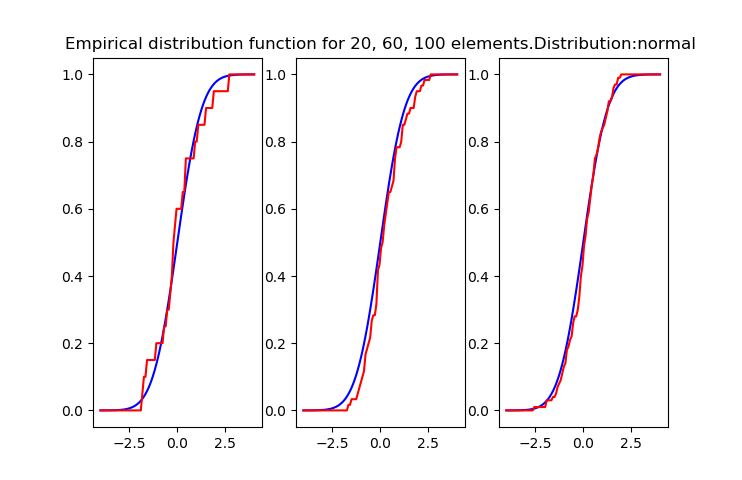
\includegraphics[width=\textwidth]{e_normal.png}
\end{figure}

\begin{figure}[H]
\caption{Эмпирическая функция для стандартного распределения Лапласа }
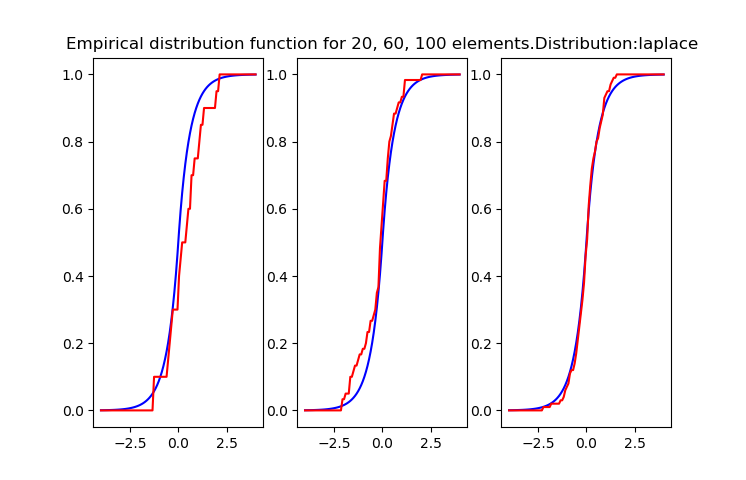
\includegraphics[width=\textwidth]{e_laplace.png} 
\end{figure}

\begin{figure}[H]
\caption{Эмпирическая функция для стандартного распределения Коши }
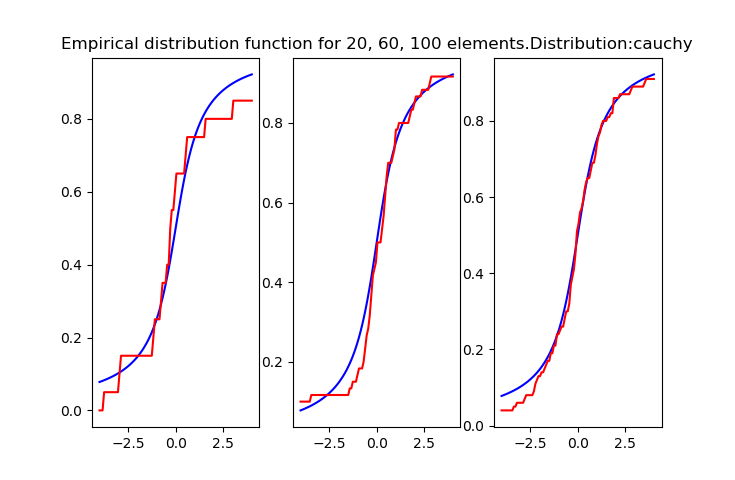
\includegraphics[width=\textwidth]{e_cauchy.png} 
\end{figure}

\begin{figure}[H]
\caption{Эмпирическая функция для распределения Пуассона }
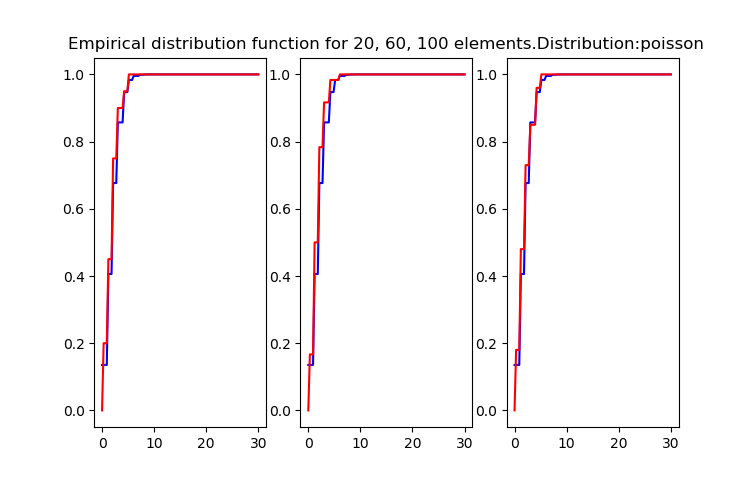
\includegraphics[width=\textwidth]{e_poisson.png} 
\end{figure}

\begin{figure}[H]
 \caption{Эмпирическая функция для равномерного распределения }
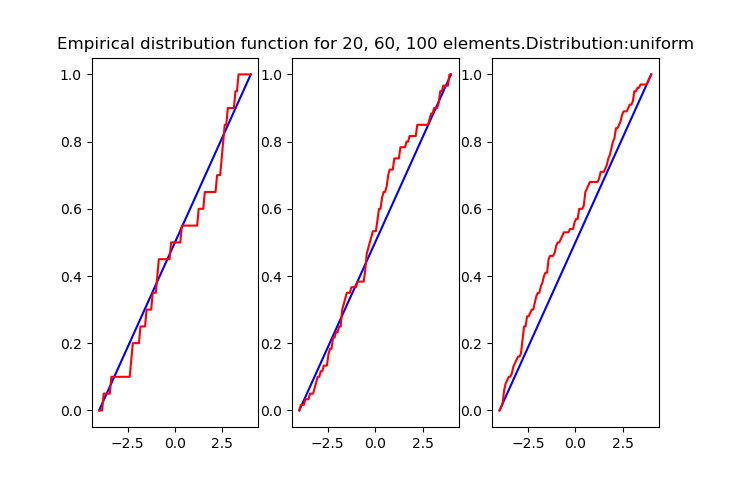
\includegraphics[width=\textwidth]{e_uniform.png}
\end{figure}
\end{center}
\subsection{Ядерные функции}

\begin{center}
    \begin{figure}[H]
 \caption{Ядерная функция плотности для нормального распределения, n = 20}
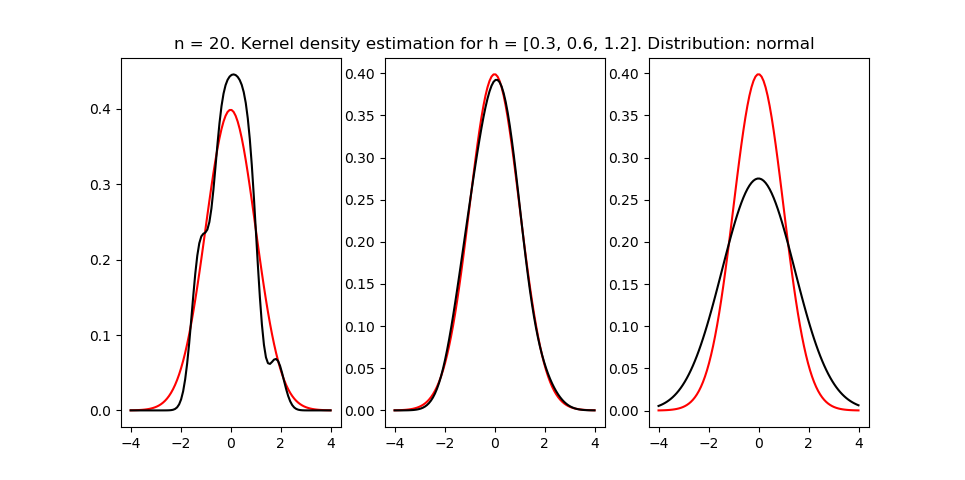
\includegraphics[width=\textwidth]{d_normal20.png}
\end{figure}
    \begin{figure}[H]
 \caption{Ядерная функция плотности для нормального распределения, n = 60}
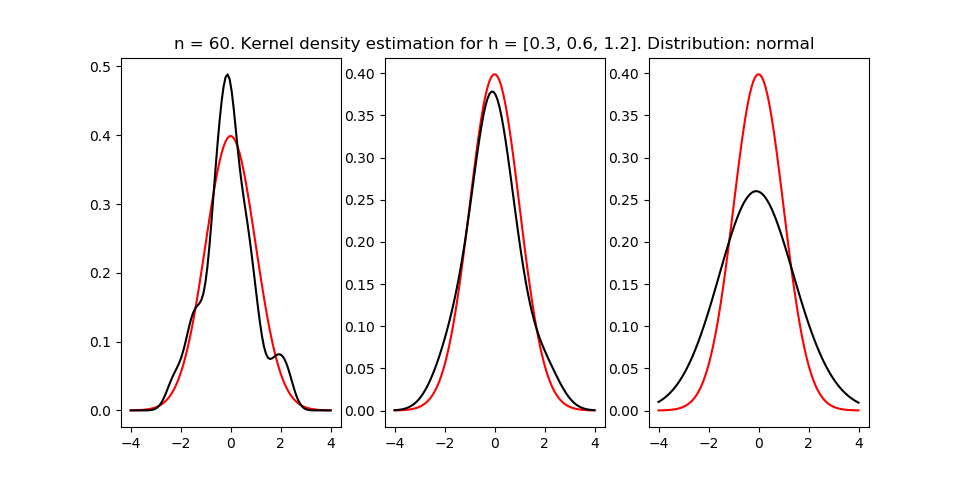
\includegraphics[width=\textwidth]{d_normal60.png}
\end{figure}
    \begin{figure}[H]
 \caption{Ядерная функция плотности для нормального распределения, n = 100}
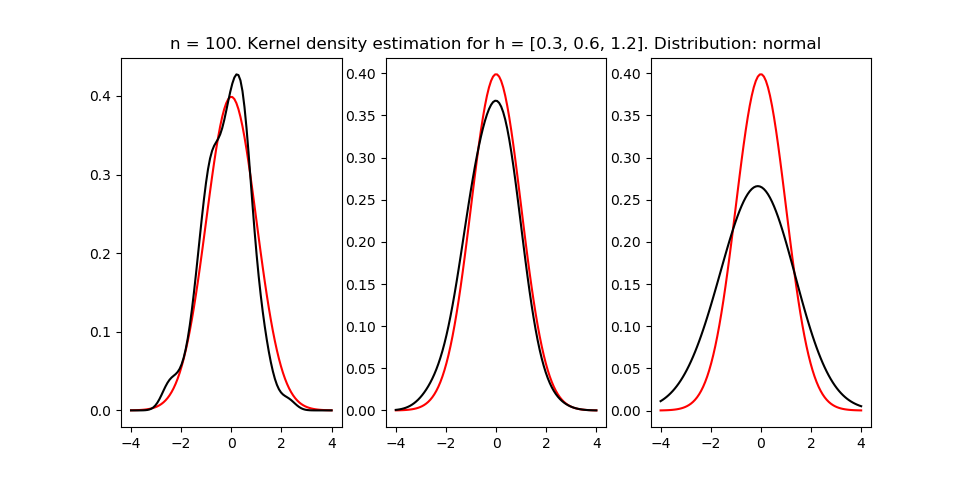
\includegraphics[width=\textwidth]{d_normal100.png}
\end{figure}

    \begin{figure}[H]
 \caption{Ядерная функция плотности для распределения Лапласа, n = 20}
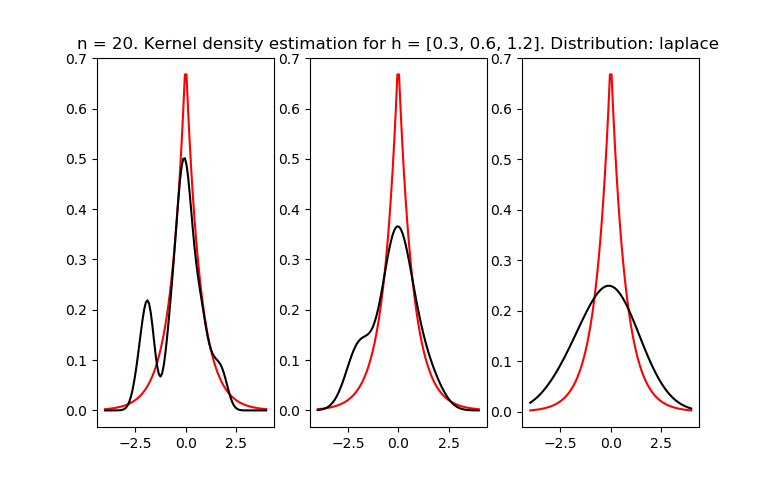
\includegraphics[width=\textwidth]{d_laplace20.png}
\end{figure}
    \begin{figure}[H]
 \caption{Ядерная функция плотности для распределения Лапласа, n = 60}
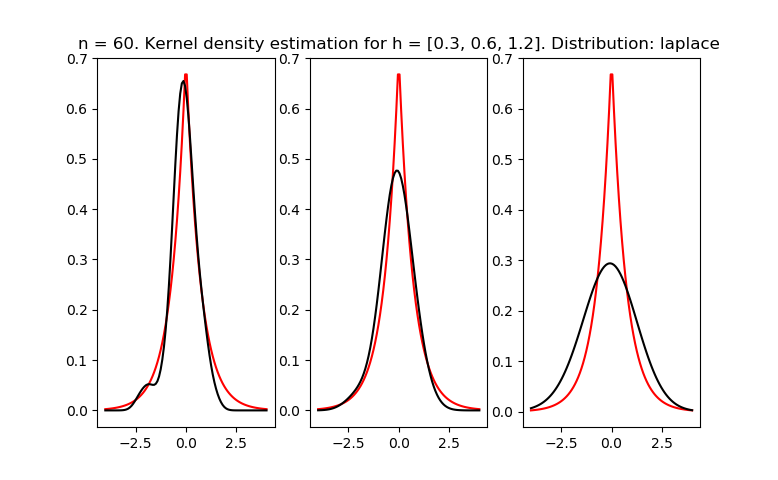
\includegraphics[width=\textwidth]{d_laplace60.png}
\end{figure}
    \begin{figure}[H]
 \caption{Ядерная функция плотности для распределения Лапласа, n = 100}
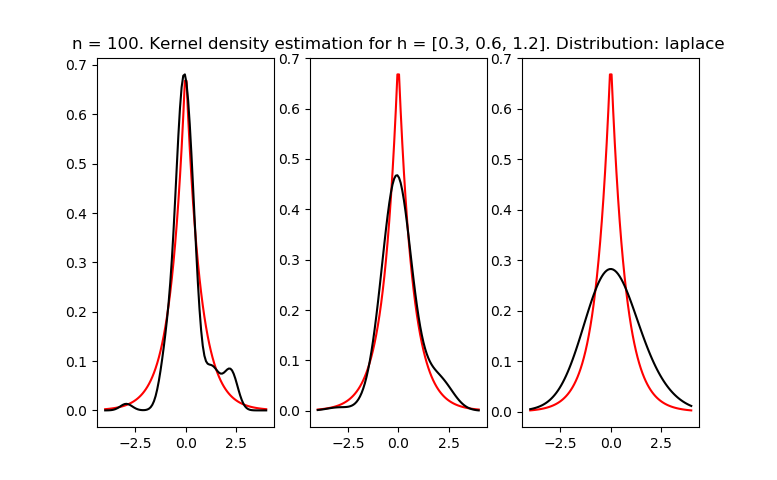
\includegraphics[width=\textwidth]{d_laplace100.png}
\end{figure}

    \begin{figure}[H]
 \caption{Ядерная функция плотности для распределения Коши, n = 20}
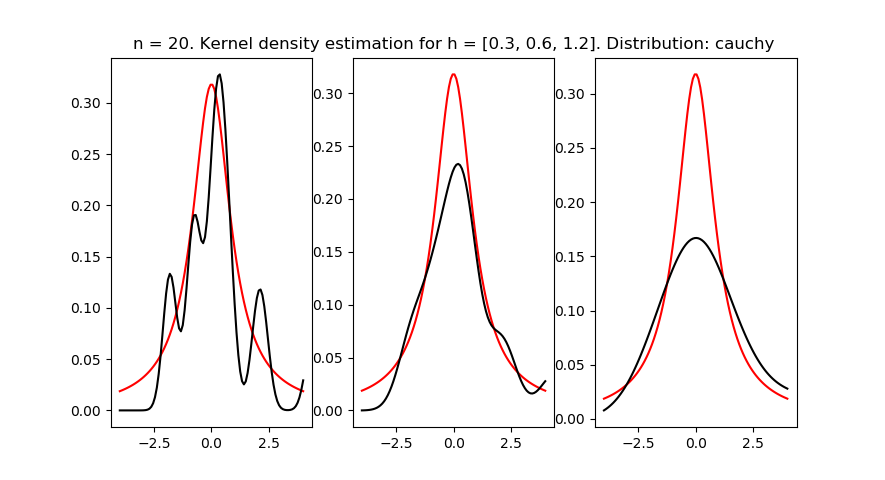
\includegraphics[width=\textwidth]{d_cauchy20.png}
\end{figure}
    \begin{figure}[H]
 \caption{Ядерная функция плотности для распределения Коши, n = 60}
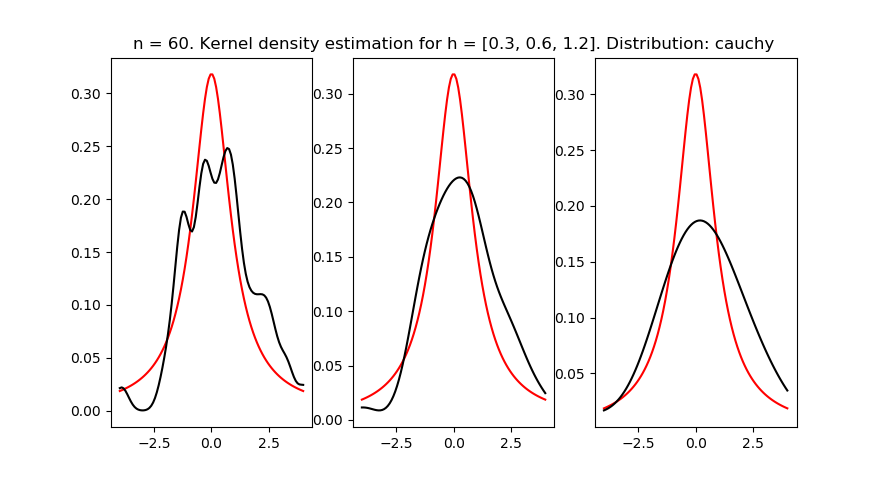
\includegraphics[width=\textwidth]{d_cauchy60.png}
\end{figure}
    \begin{figure}[H]
 \caption{Ядерная функция плотности для распределения Коши, n = 100}
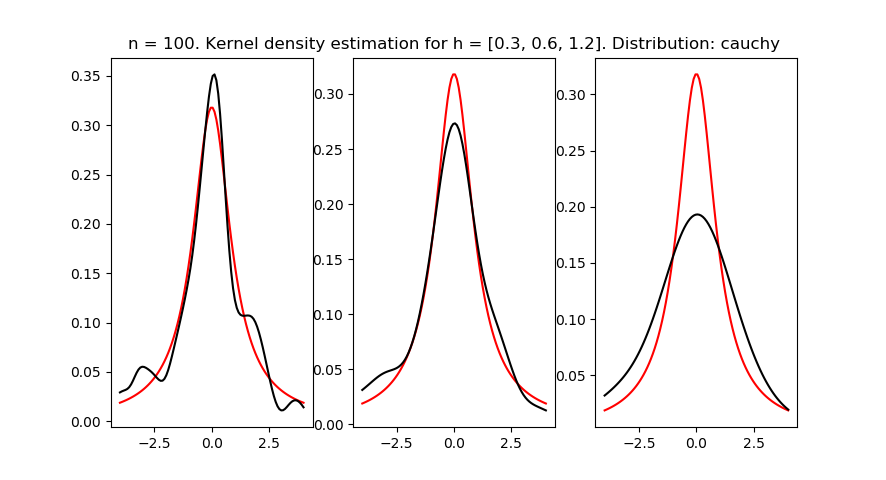
\includegraphics[width=\textwidth]{d_cauchy100.png}
\end{figure}

    \begin{figure}[H]
 \caption{Ядерная функция плотности для распределения Пуассона, n = 20}
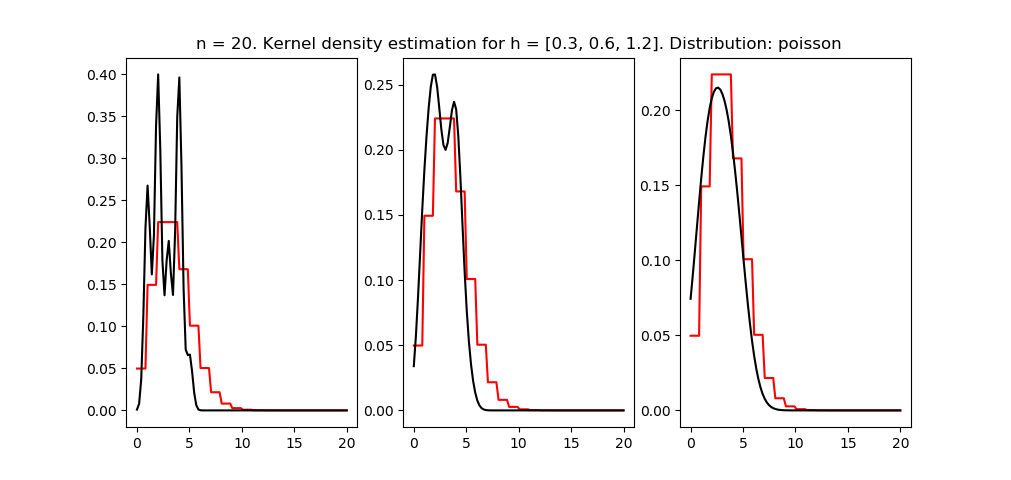
\includegraphics[width=\textwidth]{d_poisson20.png}
\end{figure}
    \begin{figure}[H]
 \caption{Ядерная функция плотности для распределения Пуассона, n = 60}
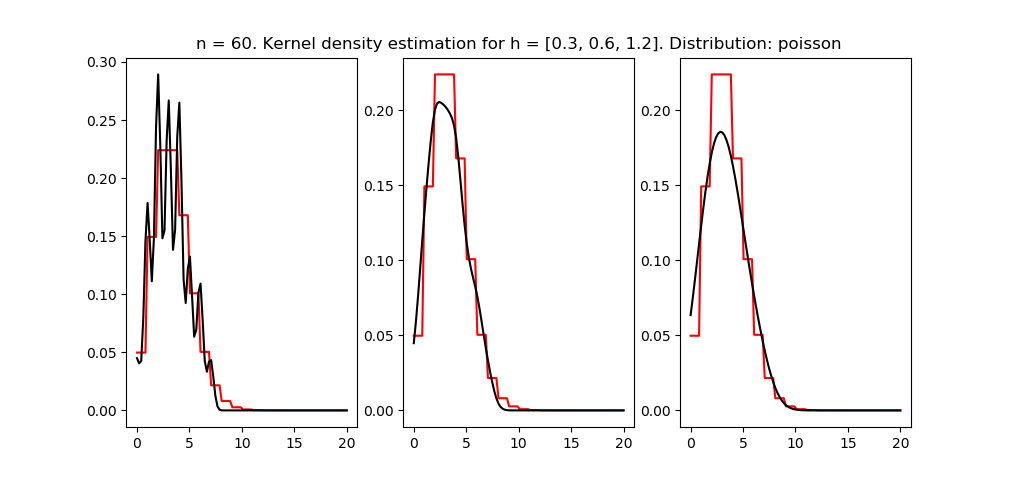
\includegraphics[width=\textwidth]{d_poisson60.png}
\end{figure}
    \begin{figure}[H]
 \caption{Ядерная функция плотности для распределения Пуассона, n = 100}
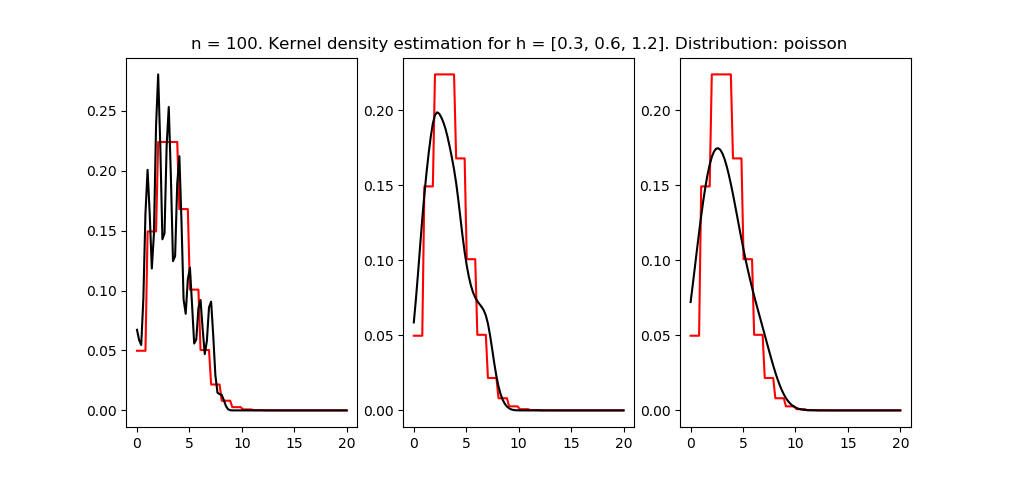
\includegraphics[width=\textwidth]{d_poisson100.png}
\end{figure}

    \begin{figure}[H]
 \caption{Ядерная функция плотности для равномерного распределения, n = 20}
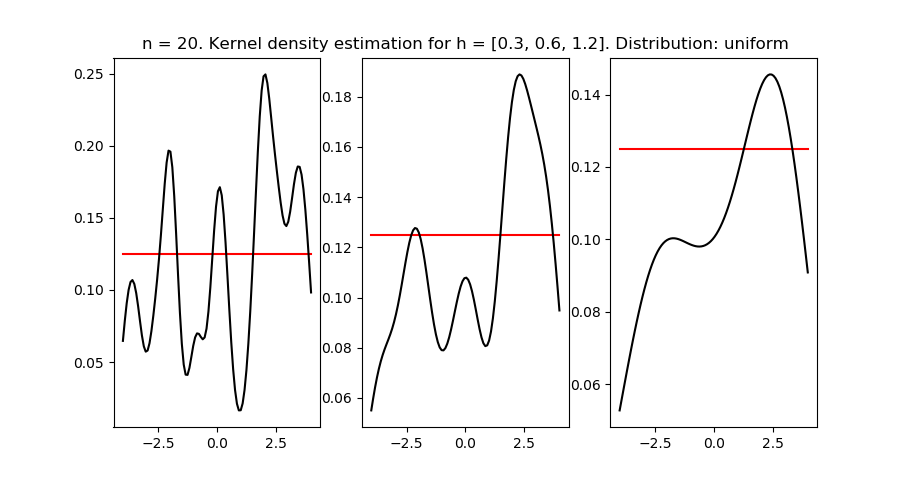
\includegraphics[width=\textwidth]{d_uniform20.png}
\end{figure}
    \begin{figure}[H]
 \caption{Ядерная функция плотности для равномерного распределения, n = 60}
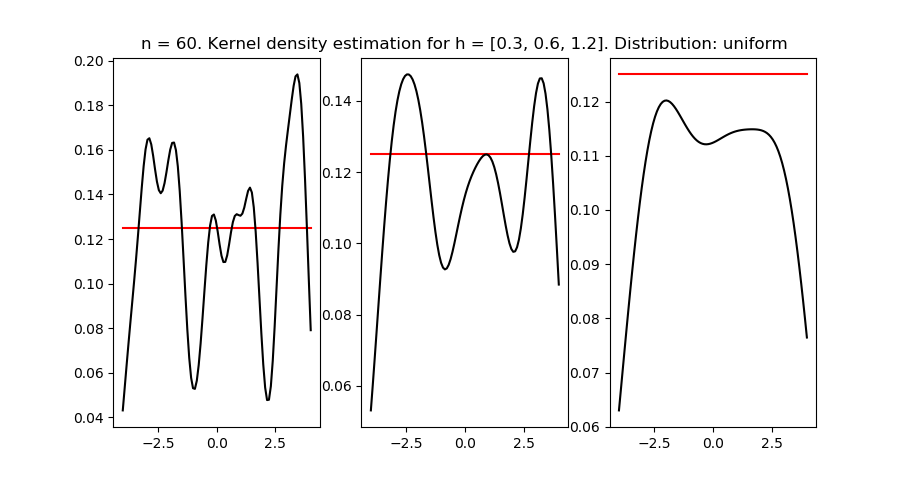
\includegraphics[width=\textwidth]{d_uniform60.png}
\end{figure}
    \begin{figure}[H]
 \caption{Ядерная функция плотности для равномерного распределения, n = 100}
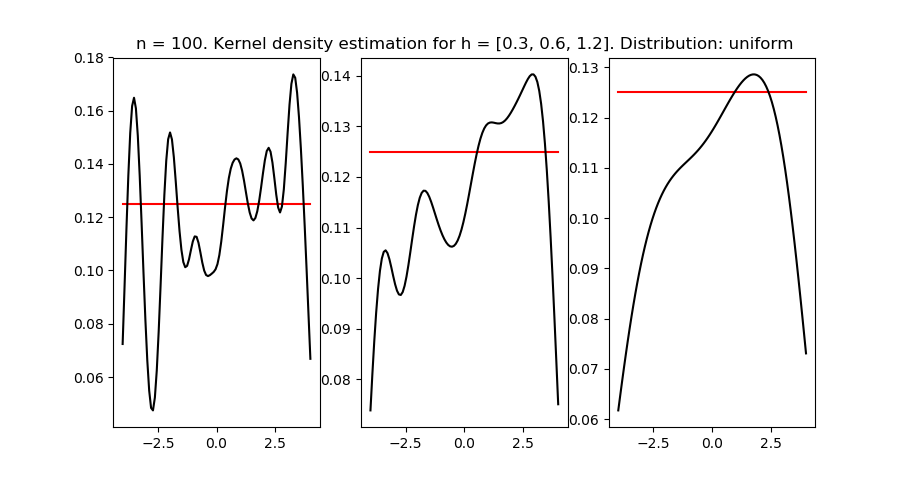
\includegraphics[width=\textwidth]{d_uniform100.png}
\end{figure}
\end{center}

\section{Выводы}
Эмпирическая функция лучше приближает эталонную функцию на больших выборках.

Наилучшее приближение функции распределения ядерной функции получено при наибольшей ширине окна. При фиксированной ширине окна точнее приблизить функцию распределения позволяет увеличение выборки.


\begin{thebibliography}{}
    \bibitem{numpy}  Модуль numpy  -  https://physics.susu.ru/vorontsov/language/numpy.html
    
    \bibitem{plotlib} 
    Модуль matplotlib - https://matplotlib.org/users/index.html
    
    \bibitem{skp}
    Модуль scipy - https://docs.scipy.org/doc/scipy/reference/
    
    \bibitem{distr_formulas}  
    Формулы распределений  -  https://vk.com/doc184549949\_491827451
    
    \bibitem{emp}  
    https://nsu.ru/mmf/tvims/chernova/ms/lec/node4.html
    
    \bibitem{art}
    https://www.mql5.com/ru/articles/396
    
    \bibitem{link:pdf}
    http://users.stat.umn.edu/~helwig/notes/den-Notes.pdf
\end{thebibliography}

\section{Приложения}


Код отчёта:\; \url{https://github.com/MisterProper9000/MatStatLabs/blob/master/MatStatLab4/MatStatLab4.tex}

Код лаборатрной:\; \url{https://github.com/MisterProper9000/MatStatLabs/blob/master/MatStatLab4/MatStatLab4.py}

\lstinputlisting[language=Python]{MatStatLab4.py}

\end{document}
